\documentclass{ximera}

%\usepackage{todonotes}

\newcommand{\todo}{}

\usepackage{tkz-euclide}
\tikzset{>=stealth} %% cool arrow head
\tikzset{shorten <>/.style={ shorten >=#1, shorten <=#1 } } %% allows shorter vectors

\usepackage{tkz-tab}  %% sign charts
\usetikzlibrary{decorations.pathreplacing} 

\usetikzlibrary{backgrounds} %% for boxes around graphs
\usetikzlibrary{shapes,positioning}  %% Clouds and stars
\usetikzlibrary{matrix} %% for matrix
\usepgfplotslibrary{polar} %% for polar plots
\usetkzobj{all}
\usepackage[makeroom]{cancel} %% for strike outs
%\usepackage{mathtools} %% for pretty underbrace % Breaks Ximera
\usepackage{multicol}

\usepackage{polynom}



\usepackage[many]{tcolorbox}  %% for titled boxes
\newtcolorbox{xbox}[1]{%
    tikznode boxed title,
    enhanced,
    arc=0mm,
    interior style={white},
    attach boxed title to top center= {yshift=-\tcboxedtitleheight/2},
    fonttitle=\bfseries,
    colbacktitle=white,coltitle=black,
    boxed title style={size=normal,colframe=white,boxrule=0pt},
    title={#1}}


\usepackage{array}
\setlength{\extrarowheight}{+.1cm}   
\newdimen\digitwidth
\settowidth\digitwidth{9}
\def\divrule#1#2{
\noalign{\moveright#1\digitwidth
\vbox{\hrule width#2\digitwidth}}}





\newcommand{\RR}{\mathbb R}
\newcommand{\R}{\mathbb R}
\newcommand{\N}{\mathbb N}
\newcommand{\Z}{\mathbb Z}

%\renewcommand{\d}{\,d\!}
\renewcommand{\d}{\mathop{}\!d}
\newcommand{\dd}[2][]{\frac{\d #1}{\d #2}}
\newcommand{\pp}[2][]{\frac{\partial #1}{\partial #2}}
\renewcommand{\l}{\ell}
\newcommand{\ddx}{\frac{d}{\d x}}
\newcommand{\ddt}{\frac{d}{\d t}}

\newcommand{\zeroOverZero}{\ensuremath{\boldsymbol{\tfrac{0}{0}}}}
\newcommand{\inftyOverInfty}{\ensuremath{\boldsymbol{\tfrac{\infty}{\infty}}}}
\newcommand{\zeroOverInfty}{\ensuremath{\boldsymbol{\tfrac{0}{\infty}}}}
\newcommand{\zeroTimesInfty}{\ensuremath{\small\boldsymbol{0\cdot \infty}}}
\newcommand{\inftyMinusInfty}{\ensuremath{\small\boldsymbol{\infty - \infty}}}
\newcommand{\oneToInfty}{\ensuremath{\boldsymbol{1^\infty}}}
\newcommand{\zeroToZero}{\ensuremath{\boldsymbol{0^0}}}
\newcommand{\inftyToZero}{\ensuremath{\boldsymbol{\infty^0}}}



\newcommand{\numOverZero}{\ensuremath{\boldsymbol{\tfrac{\#}{0}}}}
\newcommand{\dfn}{\textbf}
%\newcommand{\unit}{\,\mathrm}
\newcommand{\unit}{\mathop{}\!\mathrm}
\newcommand{\eval}[1]{\bigg[ #1 \bigg]}
\newcommand{\seq}[1]{\left( #1 \right)}
\renewcommand{\epsilon}{\varepsilon}
\renewcommand{\iff}{\Leftrightarrow}

\DeclareMathOperator{\arccot}{arccot}
\DeclareMathOperator{\arcsec}{arcsec}
\DeclareMathOperator{\arccsc}{arccsc}
\DeclareMathOperator{\si}{Si}
\DeclareMathOperator{\proj}{proj}
\DeclareMathOperator{\scal}{scal}


\newcommand{\tightoverset}[2]{% for arrow vec
  \mathop{#2}\limits^{\vbox to -.5ex{\kern-0.75ex\hbox{$#1$}\vss}}}
\newcommand{\arrowvec}[1]{\tightoverset{\scriptstyle\rightharpoonup}{#1}}
\renewcommand{\vec}{\mathbf}
\newcommand{\veci}{\vec{i}}
\newcommand{\vecj}{\vec{j}}
\newcommand{\veck}{\vec{k}}
\newcommand{\vecl}{\boldsymbol{\l}}

\newcommand{\dotp}{\bullet}
\newcommand{\cross}{\boldsymbol\times}
\newcommand{\grad}{\boldsymbol\nabla}
\newcommand{\divergence}{\grad\dotp}
\newcommand{\curl}{\grad\cross}
%\DeclareMathOperator{\divergence}{divergence}
%\DeclareMathOperator{\curl}[1]{\grad\cross #1}


\colorlet{textColor}{black} 
\colorlet{background}{white}
\colorlet{penColor}{blue!50!black} % Color of a curve in a plot
\colorlet{penColor2}{red!50!black}% Color of a curve in a plot
\colorlet{penColor3}{red!50!blue} % Color of a curve in a plot
\colorlet{penColor4}{green!50!black} % Color of a curve in a plot
\colorlet{penColor5}{orange!80!black} % Color of a curve in a plot
\colorlet{fill1}{penColor!20} % Color of fill in a plot
\colorlet{fill2}{penColor2!20} % Color of fill in a plot
\colorlet{fillp}{fill1} % Color of positive area
\colorlet{filln}{penColor2!20} % Color of negative area
\colorlet{fill3}{penColor3!20} % Fill
\colorlet{fill4}{penColor4!20} % Fill
\colorlet{fill5}{penColor5!20} % Fill
\colorlet{gridColor}{gray!50} % Color of grid in a plot

\newcommand{\surfaceColor}{violet}
\newcommand{\surfaceColorTwo}{redyellow}
\newcommand{\sliceColor}{greenyellow}




\pgfmathdeclarefunction{gauss}{2}{% gives gaussian
  \pgfmathparse{1/(#2*sqrt(2*pi))*exp(-((x-#1)^2)/(2*#2^2))}%
}


%%%%%%%%%%%%%
%% Vectors
%%%%%%%%%%%%%

%% Simple horiz vectors
\renewcommand{\vector}[1]{\left\langle #1\right\rangle}


%% %% Complex Horiz Vectors with angle brackets
%% \makeatletter
%% \renewcommand{\vector}[2][ , ]{\left\langle%
%%   \def\nextitem{\def\nextitem{#1}}%
%%   \@for \el:=#2\do{\nextitem\el}\right\rangle%
%% }
%% \makeatother

%% %% Vertical Vectors
%% \def\vector#1{\begin{bmatrix}\vecListA#1,,\end{bmatrix}}
%% \def\vecListA#1,{\if,#1,\else #1\cr \expandafter \vecListA \fi}

%%%%%%%%%%%%%
%% End of vectors
%%%%%%%%%%%%%

%\newcommand{\fullwidth}{}
%\newcommand{\normalwidth}{}



%% makes a snazzy t-chart for evaluating functions
%\newenvironment{tchart}{\rowcolors{2}{}{background!90!textColor}\array}{\endarray}

%%This is to help with formatting on future title pages.
\newenvironment{sectionOutcomes}{}{} 



%% Flowchart stuff
%\tikzstyle{startstop} = [rectangle, rounded corners, minimum width=3cm, minimum height=1cm,text centered, draw=black]
%\tikzstyle{question} = [rectangle, minimum width=3cm, minimum height=1cm, text centered, draw=black]
%\tikzstyle{decision} = [trapezium, trapezium left angle=70, trapezium right angle=110, minimum width=3cm, minimum height=1cm, text centered, draw=black]
%\tikzstyle{question} = [rectangle, rounded corners, minimum width=3cm, minimum height=1cm,text centered, draw=black]
%\tikzstyle{process} = [rectangle, minimum width=3cm, minimum height=1cm, text centered, draw=black]
%\tikzstyle{decision} = [trapezium, trapezium left angle=70, trapezium right angle=110, minimum width=3cm, minimum height=1cm, text centered, draw=black]


\title[Dig-In:]{The Intermediate Value Theorem}

\outcome{State the Intermediate Value Theorem including hypotheses.}
\outcome{Sketch pictures indicating why the Intermediate Value Theorem is true, and why all hypotheses are necessary.}
\outcome{Explain why certain points exist using the Intermediate Value Theorem.}


\begin{document}

\begin{abstract}
  Here we see a consequence of a function being continuous.
\end{abstract}
\maketitle



The \textit{Intermediate Value Theorem} should not be brushed off
lightly. Once it is understood, it may seem ``obvious,'' but
mathematicians should not underestimate its power.

\begin{theorem}[Intermediate Value Theorem]\label{theorem:IVT}\index{Intermediate Value Theorem}
	If $f$ is a continuous function for all $x$ in the closed interval
	$[a,b]$ and $L$ is between $f(a)$ and $f(b)$, then there is a number
	$c$ in $[a, b]$ such that $f(c) = L$.
\end{theorem}

%% \marginnote[-1.2in]{The Intermediate Value Theorem is most frequently
%%   used when $d=0$.}  
%% \marginnote[-.7in]{For a nice proof of this theorem, see: Walk, Stephen
%%   M. \textit{The intermediate value theorem is NOT obvious---and I am
%%     going to prove it to you}. College Math. J. 42 (2011), no. 4,
%%   254--259.}
%% In Figure~\ref{figure:intermediate-value}, we see a geometric
%% interpretation of this theorem.
%%BADBAD here we have a note on the proof, see the source


\begin{image}
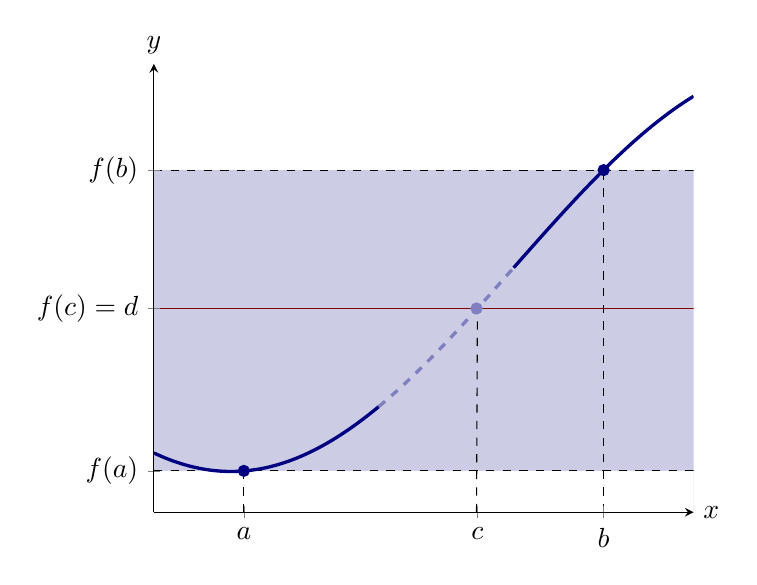
\begin{tikzpicture}
	\begin{axis}[
            domain=0:6, ymin=0, ymax=2.2,xmax=6,
            axis lines =left, xlabel=$x$, ylabel=$y$,
            every axis y label/.style={at=(current axis.above origin),anchor=south},
            every axis x label/.style={at=(current axis.right of origin),anchor=west},
            xtick={1,3.597,5}, ytick={.203,1,1.679},
            xticklabels={$a$,$c$,$b$}, yticklabels={$f(a)$,$f(c)=d$,$f(b)$},
            axis on top,
          ]
          \addplot [draw=none, fill=fill1, domain=(0:7)] {1.679} \closedcycle;
          \addplot [draw=none, fill=background, domain=(0:7)] {.203} \closedcycle;
          \addplot [textColor,dashed] plot coordinates {(0,1.679) (6,1.679)};
          \addplot [textColor,dashed] plot coordinates {(0,.203) (6,.203)};
          \addplot [textColor,dashed] plot coordinates {(5,0) (5,1.679)};
          \addplot [textColor,dashed] plot coordinates {(1,0) (1,.203)};
          \addplot [textColor,dashed] plot coordinates {(3.587,0) (3.597,1)};
          \addplot [penColor2,domain=(0:6)] {1};
          \addplot [very thick,penColor, smooth,domain=(0:2.5)] {sin(deg((x - 4)/2)) + 1.2};
          \addplot [very thick,penColor, smooth,domain=(4:6)] {sin(deg((x - 4)/2)) + 1.2};
          \addplot [very thick,dashed,penColor!50!background, smooth,domain=(2.5:4)] {sin(deg((x - 4)/2)) + 1.2}; 
          \addplot [color=penColor!50!background,fill=penColor!50!background,only marks,mark=*] coordinates{(3.587,1)};  %% closed hole          
          \addplot [color=penColor,fill=penColor,only marks,mark=*] coordinates{(1,.203)};  %% closed hole          
          \addplot [color=penColor,fill=penColor,only marks,mark=*] coordinates{(5,1.679)};  %% closed hole          
        \end{axis}
\end{tikzpicture}
%% \caption{A geometric interpretation of the Intermediate Value
%%   Theorem. The function $f(x)$ is continuous on the interval
%%   $[a,b]$. Since $L$ is in the interval $[f(a),f(b)]$, there exists a
%%   value $c$ in $[a,b]$ such that $f(c) = L$.}
%% \label{figure:intermediate-value}
\end{image}

Now, let's contrast this with a time when the conclusion of the
Intermediate Value Theorem does not hold.

\begin{question}
  Consider the following situation,
  \begin{image}
    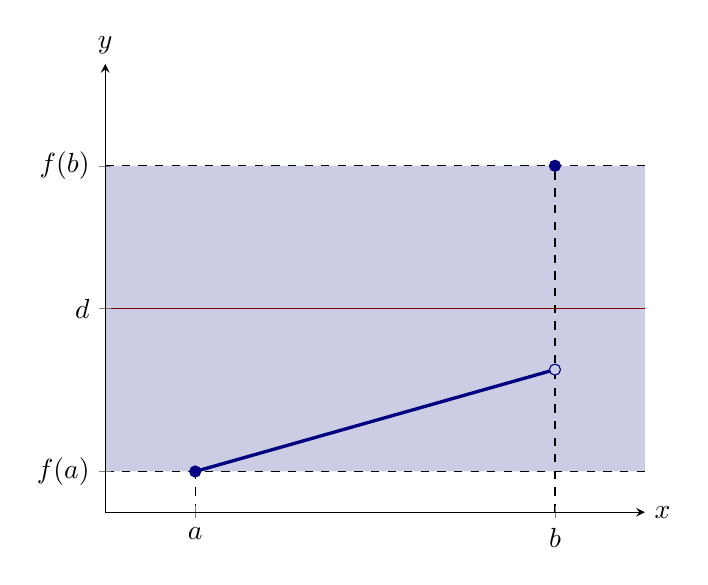
\begin{tikzpicture}
      \begin{axis}[
          domain=0:6, ymin=0, ymax=2.2,xmax=6,
          axis lines =left, xlabel=$x$, ylabel=$y$,
          every axis y label/.style={at=(current axis.above origin),anchor=south},
          every axis x label/.style={at=(current axis.right of origin),anchor=west},
          xtick={1,5}, ytick={.2,1,1.7},
          xticklabels={$a$,$b$}, yticklabels={$f(a)$,$d$,$f(b)$},
          axis on top,
        ]
        \addplot [draw=none, fill=fill1, domain=(0:7)] {1.7} \closedcycle;
        \addplot [draw=none, fill=background, domain=(0:7)] {.2} \closedcycle;
        \addplot [textColor,dashed] plot coordinates {(0,1.7) (6,1.7)};
        \addplot [textColor,dashed] plot coordinates {(0,.2) (6,.2)};
        \addplot [textColor,dashed] plot coordinates {(5,0) (5,1.7)};
        \addplot [textColor,dashed] plot coordinates {(1,0) (1,.2)};
        \addplot [penColor2,domain=(0:6)] {1};
        \addplot [very thick,penColor] plot coordinates {(1,.2) (5,.7)};
        \addplot [color=penColor,fill=penColor,only marks,mark=*] coordinates{(1,.2)};  %% closed hole
        \addplot [color=penColor,fill=fill1,only marks,mark=*] coordinates{(5,.7)};  %% open hole          
        \addplot [color=penColor,fill=penColor,only marks,mark=*] coordinates{(5,1.7)};  %% closed hole          
      \end{axis}
    \end{tikzpicture}
  \end{image}
  and select all that are true:
  \begin{selectAll}
    \choice[correct]{$f$ is continuous on $(a,b)$.}
    \choice[correct]{$f$ is continuous on $[a,b)$.}
    \choice{$f$ is continuous on $(a,b]$.}
    \choice{$f$ is continuous on $[a,b]$.}
    \choice{There is a point $c$ in $[a,b]$ with $f(c) = L$.}
  \end{selectAll}
\end{question}

Building on the question above, it is not difficult to see that 
each of the hypothesis of the Intermediate Value Theorem are necessary.



Let's see the Intermediate Value Theorem in action.


\begin{example}
Explain why the function $f(x)=x^3 + 3x^2+x-2$ has a root between $0$
and $1$.


\begin{explanation}
Since $f$ is a polynomial, we see that $f$ is continuous for all real
numbers.  Since $f(0)=\answer[given]{-2}$ and
$f(1)=\answer[given]{3}$, and $0$ is between $-2$ and $3$, by the
Intermediate Value Theorem, there is a point $c$ in the interval
$[0,1]$ such that $f(c)=\answer[given]{0}$.
\end{explanation}
\end{example}



This example also points the way to a simple method for approximating
roots. 



\begin{example} 
Approximate a root of $f(x) =x^3 + 3x^2+x-2$ between $0$ and $1$ to
within one decimal place.

\begin{explanation} 
Again, since $f$ is a polynomial, we see that $f$ is continuous for
all real numbers. Compute
\[
\begin{array}{c|c}
  x   & f(x) \\ \hline
  0.1 & \answer[given]{-1.869}\\
  0.2 & \answer[given]{-1.672}\\
  0.3 & \answer[given]{-1.403}\\
  0.4 & \answer[given]{-1.056}\\
  0.5 & \answer[given]{-0.625}\\
  0.6 & \answer[given]{-0.104}\\
  0.7 & \answer[given]{0.513}
\end{array}
\]
By the Intermediate Value Theorem, $f$ has a root between $0.6$ and
$0.7$. Repeating the process
\[
\begin{array}{c|c}
  x   & f(x) \\ \hline
  0.61 & \answer[given]{-0.046719}\\
  0.62 & \answer[given]{0.011528}
\end{array}
\]
so by the Intermediate Value Theorem, $f$ has a root between $0.61$
and $0.62$, and the root is $0.6$ rounded to one decimal place.
\end{explanation}
\end{example}


The Intermediate Value Theorem can be use to show that curves cross:


\begin{example} 
  Explain why the functions
  \begin{align*}
    f(x) &= x^2\sqrt[3]{x}\\
    g(x) &= 2(x+1)\cos(\sqrt[3]{x})
  \end{align*}
  intersect on the interval $\left[0,\left( \frac{\pi}{2}\right)^3 \right]$.

  To start, note that both $f$ and $g$ are continuous functions, and
  hence $h = f-g$ is also a continuous function. Now
  \begin{align*}
    h(0) &= f(0) - g(0) \\
    &= (\answer[given]{0})^2\cdot \sqrt[3]{(\answer[given]{0})} - 2\cdot(\answer[given]{0}+1) \cdot \cos\left(\sqrt[3]{(\answer[given]{0})} \right)\\
    &= \answer[given]{-2}.
  \end{align*}
  and in a similar fashion
   \begin{align*}
    h\left(\left( \frac{\pi}{2}\right)^3\right) &= f\left(\left( \frac{\pi}{2}\right)^3\right) - g\left(\left( \frac{\pi}{2}\right)^3\right) \\
         &= \left( \left( \frac{\pi}{2}\right)^3\right)^2\cdot \sqrt[3]{\left( \frac{\pi}{2}\right)^3} \\ 
         & -  2\cdot\left( \left( \frac{\pi}{2}\right)^3+1\right) \cdot \cos\left(\sqrt[3]{\left( \frac{\pi}{2}\right)^3} \right)\\
   \end{align*}
   Since $\cos\left( \frac{\pi}{2}\right)=0$ we see that the expression above is
   positive. Hence by the Intermediate Value Theorem, $f$ and $g$
   intersect on the interval $\left[0,\left( \frac{\pi}{2}\right)^3 \right]$.
   \begin{onlineOnly}
   We can see this point of intersection by looking at the graphs of $y=f(x)$ and $y=g(x)$ on the given interval. 
   \[
   \graph[xmin=1,xmax=e,ymin=-10,ymax=10]{x^2 *x^(1/3), 2(x+1)\cos(x^(1/3))}
   \]
   \end{onlineOnly}
\end{example}




Now we move on to a more subtle example:

\begin{example}
Suppose you have two cats, Roxy and Yuri. Is there a time when Roxy
and Yuri have the same amount of water in their bowls assuming:
  \begin{itemize}
  \item They start and finish drinking at the same times.
  \item Roxy starts with more water than Yuri, and leaves less water
    left in her bowl than Yuri.
  \end{itemize}

\begin{explanation} 
  To solve this problem, consider two functions:
  \begin{itemize}
    \item $W_{\mathrm{Roxy}}(t) =$ the amount of water in Roxy's bowl at time $t$.
    \item $W_{\mathrm{Yuri}}(t) =$ the amount of water in Yuri's bowl at time $t$.
  \end{itemize}
  Now if $t_\mathrm{start}$ is the time the cats start drinking and
  $t_\mathrm{finish}$ is the time the cats finish drinking. Then we have
  \[
  W_\mathrm{Roxy}(t_\mathrm{start})-W_{\mathrm{Yuri}}(t_\mathrm{start}) > 0%%BADBAD dropdown answer type wanted for < > =
  \]
  and
  \[
  W_\mathrm{Roxy}(t_\mathrm{finish})-W_{\mathrm{Yuri}}(t_\mathrm{finish}) < 0.
  \]
  Since the amount of water in a bowl at time $t$ is a continuous
  function, as water is ``lapped'' up in continuous amounts,
  \[
  W_\mathrm{Roxy}-W_{\mathrm{Yuri}}
  \]
  is a continuous function, and hence the Intermediate Value Theorem
  applies. Since $W_\mathrm{Roxy}-W_{\mathrm{Yuri}}$ is positive when
  at $t_\mathrm{start}$ and negative at $t_\mathrm{finish}$, there is
  some time $t_\mathrm{equal}$ when the value is zero, meaning
  \[
  W_\mathrm{Roxy}(t_\mathrm{equal})-  W_{\mathrm{Yuri}}(t_\mathrm{equal}) =0
  \]
  meaning there is the same amount of water in each of their bowls.
\end{explanation}
\end{example}


And finally, an example when the Intermediate Value Theorem
\textit{does not} apply.


\begin{example}
Suppose you have two cats, Roxy and Yuri. Is there a time when Roxy
and Yuri have the same amount of dry cat food in their bowls assuming:
  \begin{itemize}
  \item They start and finish eating at the same times.
  \item Roxy starts with more food than Yuri, and leaves less food
    uneaten than Yuri.
  \end{itemize}

\begin{explanation} 
  Here we could try the same approach as before, setting:
  \begin{itemize}
    \item $F_{\mathrm{Roxy}}(t) =$ the amount of dry cat food in Roxy's bowl at time $t$.
    \item $F_{\mathrm{Yuri}}(t) =$ the amount of dry cat food in Yuri's bowl at time $t$.
  \end{itemize}
  However in this case, the amount of food in a bowl at time $t$ is
  \textbf{not} a continuous function! This is because dry cat food
  consists of discrete kibbles, and is not eaten in a continuous
  fashion. Hence the Intermediate Value Theorem \textbf{does not
    apply}, and we can make no definitive statements concerning the
  question above.
\end{explanation}
\end{example}


\end{document}
